%%%%%%%%%%%%%%%%%%%%%%%%%%%%%%%%%%%%%%%%%%%%%%%%%%%%%%%%%%%%%%%%%%%%%%%%%%%%%%
%
% Appendix file included in main project file using \input{}
%
% Assumes that LaTeX2e macros and packages defined in cg_comp.sty are
%   available
%
%%%%%%%%%%%%%%%%%%%%%%%%%%%%%%%%%%%%%%%%%%%%%%%%%%%%%%%%%%%%%%%%%%%%%%%%%%%%%%

 \section{Fretting Classical Guitar Strings\label{app:fret}}

\begin{figure}
    \centering
    \begin{subfigure}[b]{0.45\textwidth}
        \centering
        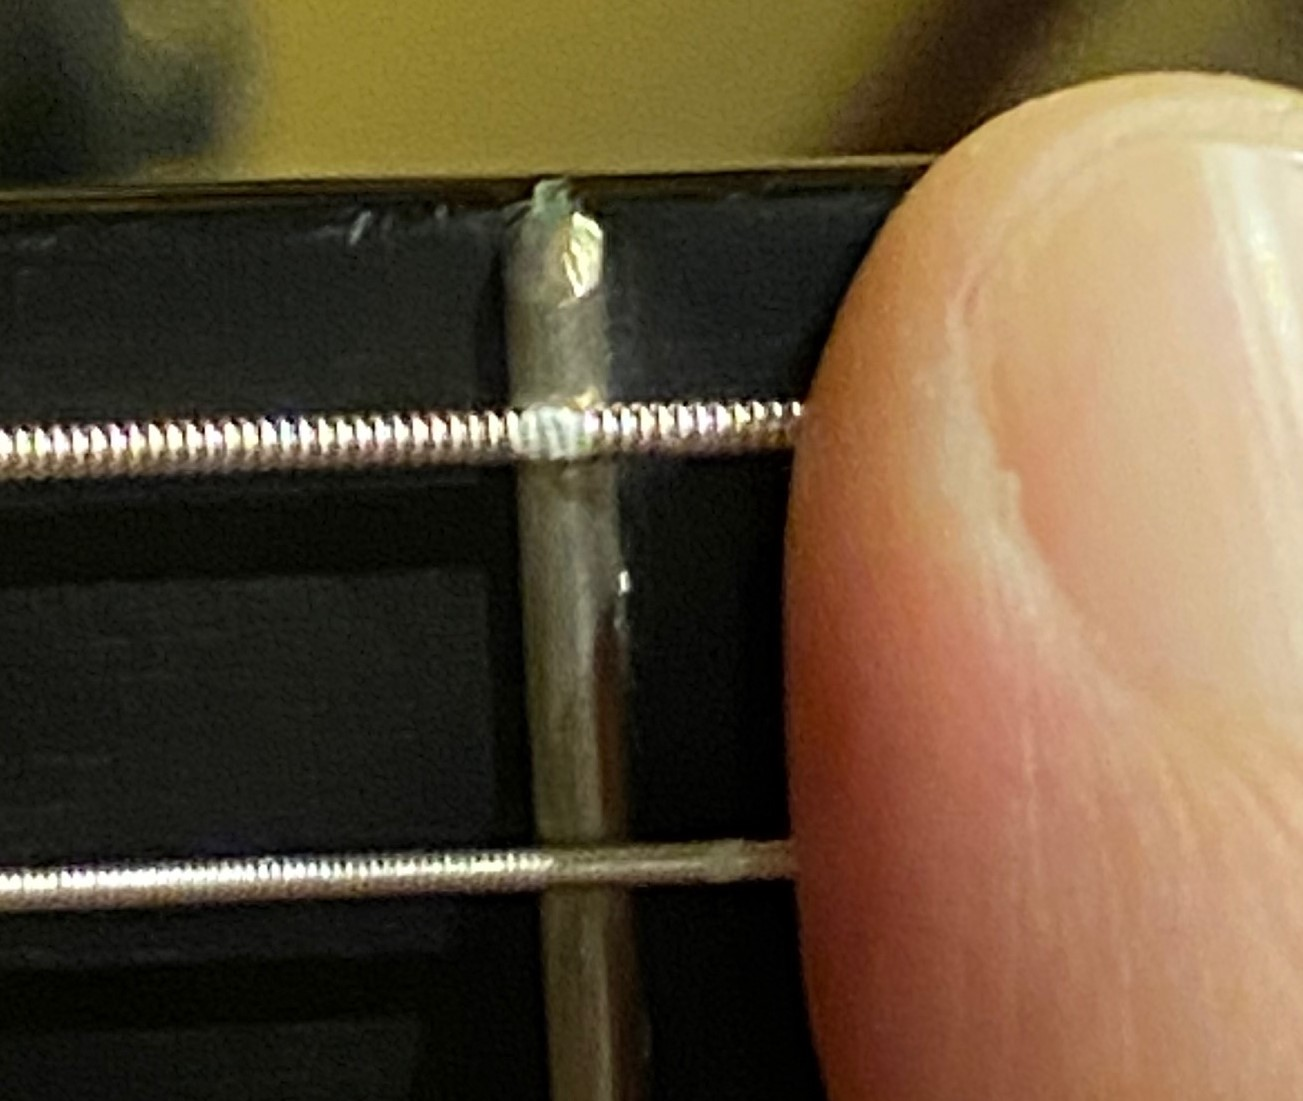
\includegraphics[width=3.0in]{figures/fret_before.jpg}
        \caption{Before fretting}
        \label{fig:fret_before}
    \end{subfigure}
    \hspace{0.25in}
    \begin{subfigure}[b]{0.45\textwidth}
        \centering
        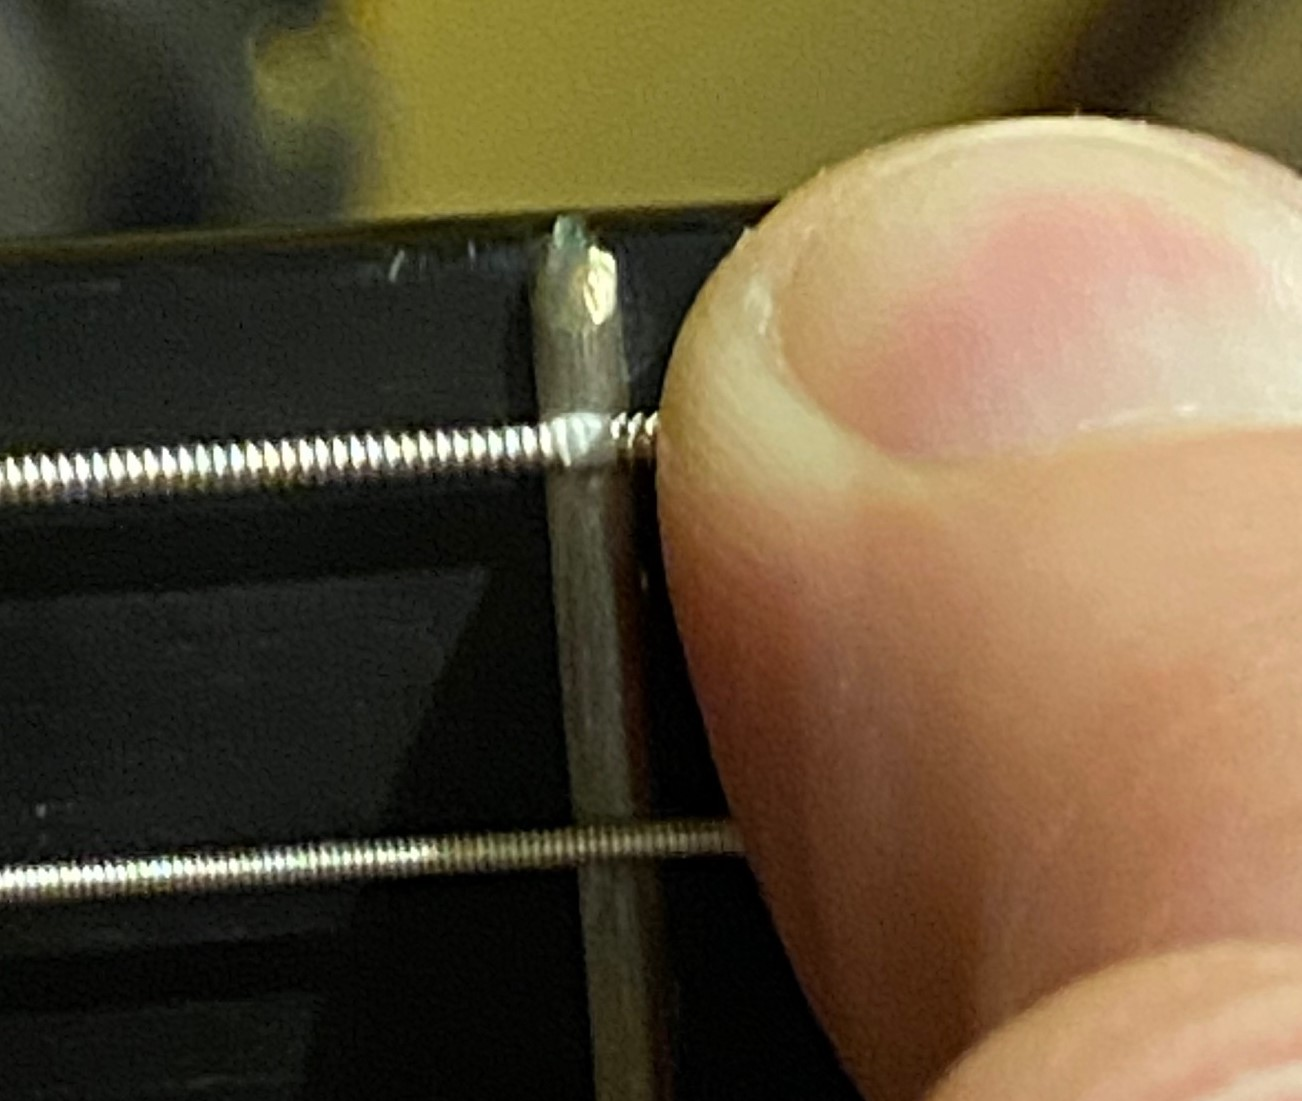
\includegraphics[width=3.04in]{figures/fret_after.jpg}
        \caption{After fretting}
        \label{fig:fret_after}
    \end{subfigure}
    \caption{\label{fig:fret_befaft} Location of a small marker of white correction fluid before and after fretting.}
  \end{figure}
  
Previous studies of guitar intonation and compensation~\cite{ref:byers1996cgi,ref:varieschi2010icf} included a contribution to the incremental change in the length of the fretted string caused by both the depth and the shape of the string under the finger. As the string is initially pressed to the fret, the total length $\mathcal{L}_n$ increases and causes the tension in the string to increase. When the string is pressed further, does the additional deformation of the string increase its tension (throughout the resonant length $L_n$)? There are at least two purely empirical reasons to doubt this hypothesis. First, as shown in \fig{fret_befaft}, we can mark a string (with a small deposit of white correction fluid) above a particular fret and then observe the mark with a magnifying glass. As the string is pressed flat on the finger board with two fingers, the mark does not move perceptibly --- it has become \emph{clamped} on the fret. Second, we can use either our ears or a simple tool to measure frequencies~\cite{ref:pgtweb} to listen for a shift as we apply different fingers and vary the fretted depth of a string. The apparent modulation is far less than would be obtained by classical vibrato ($\pm15$~cents) --- which causes the mark on the string to move visibly --- so we assume that once the string is minimally fretted the length(s) can be regarded as fixed. (If this were not the case, then fretting by different people or with different fingers, at a single string or with a barre, would cause additional, varying frequency shifts that would be audible and difficult to compensate.)

\begin{figure}
    \centering
    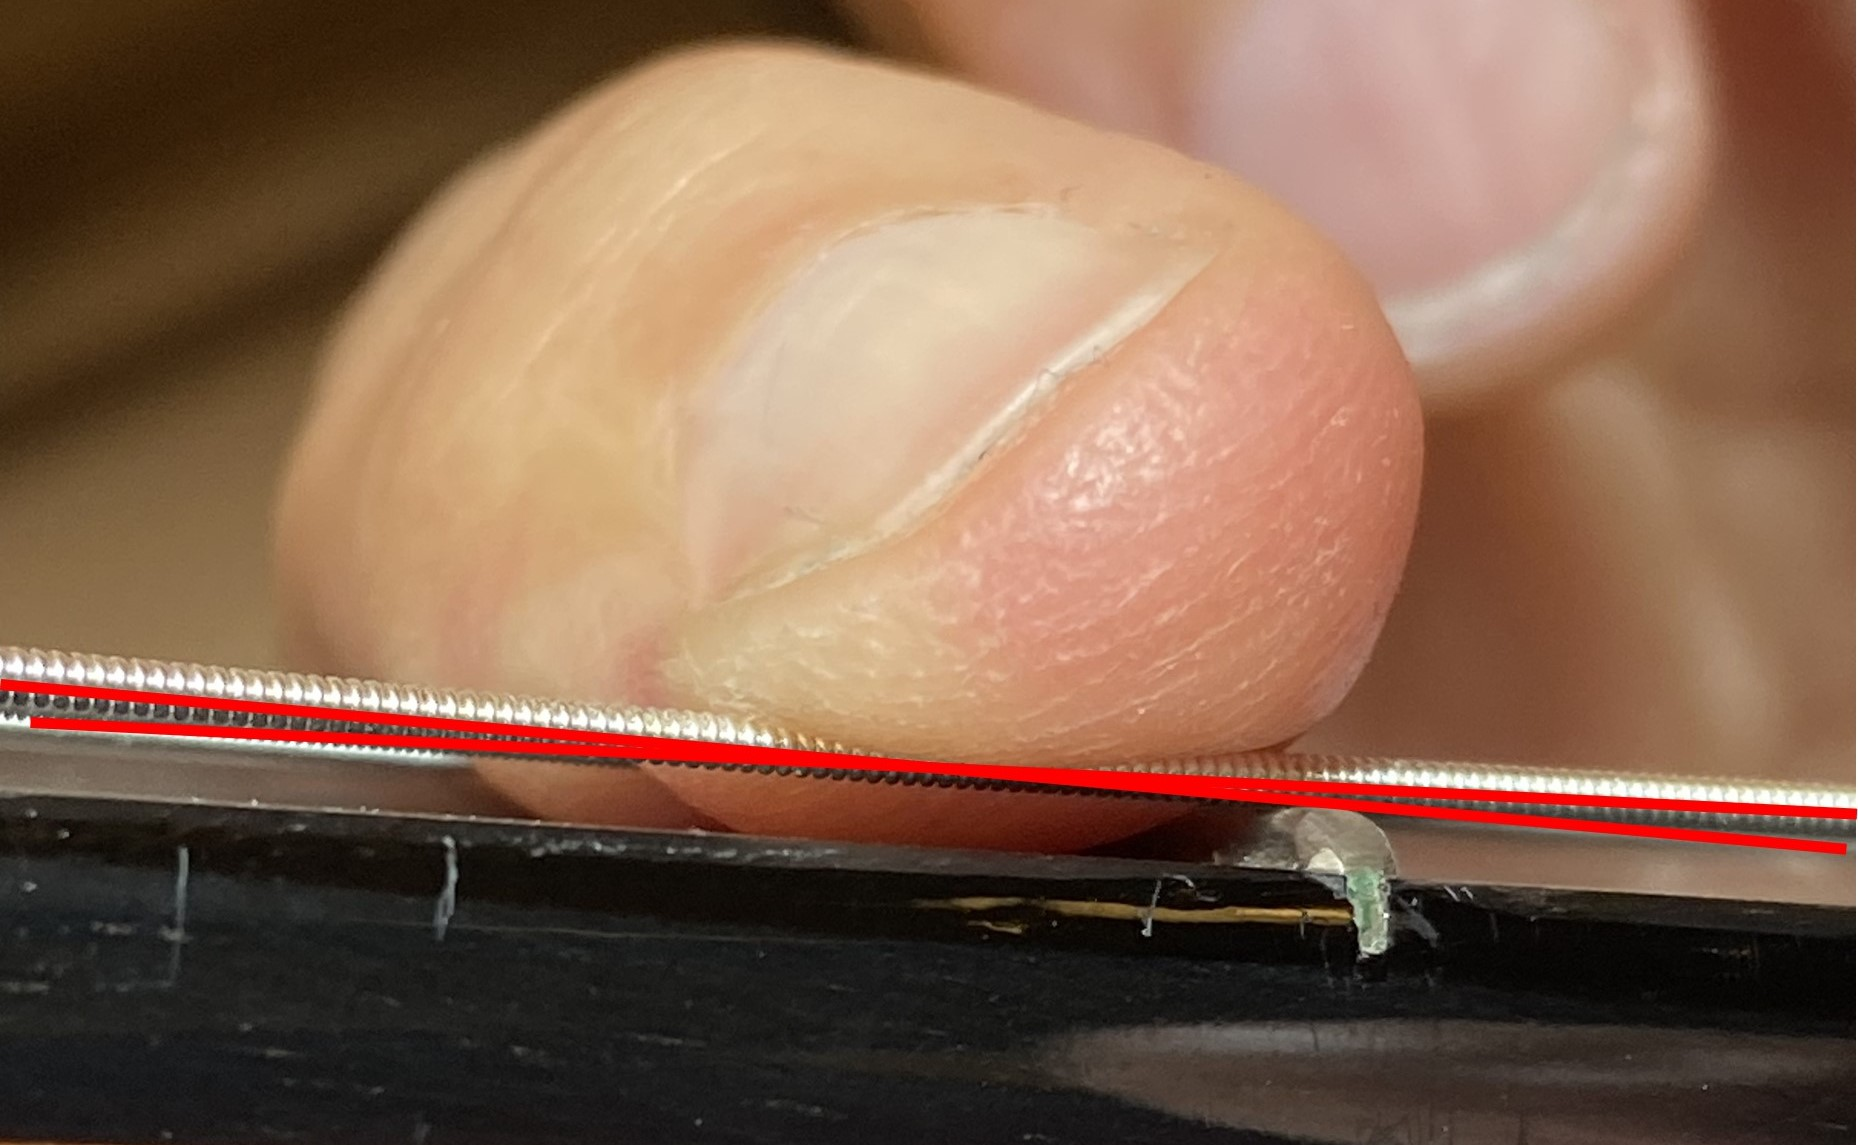
\includegraphics[width=6.0in]{figures/fretting_photo}
    \caption{\label{fig:fretting_photo} Photo of a wound nylon $E_2$ string clamped at the first fret of a classical guitar. The shape of the fretted string can be well approximated by two line segments intersecting about 5--6~mm behind the fret.}
\end{figure}

% \begin{figure}
%     \centering
%     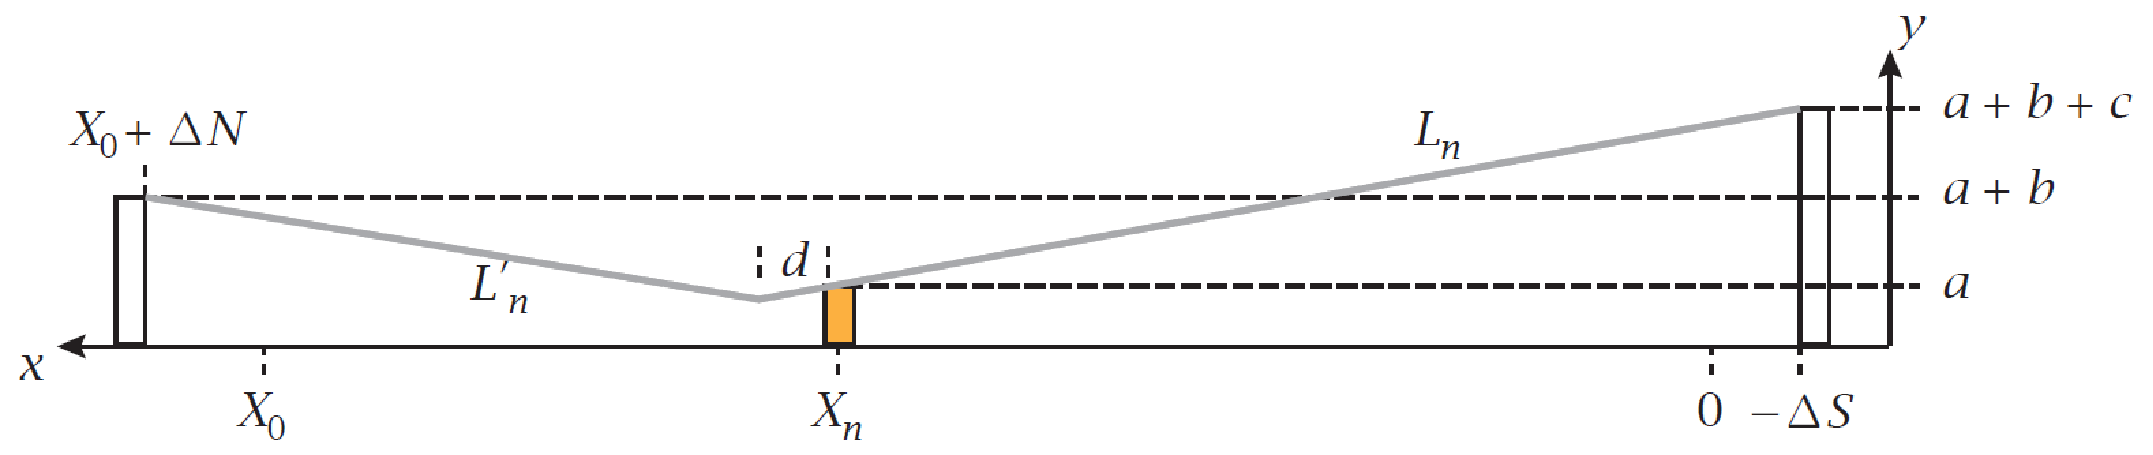
\includegraphics[width=6.0in]{figures/fretting_schematic}
%     \caption{\label{fig:fretting_schematic} A recapitulation of \fig{guitar_schematic} with the addition of a line-segment intersection at a distance $d$ behind fret $n$ to represent the slight increase in the distance $L_n^\prime$ caused by a finger.}
% \end{figure}

In \sct{model}, we have included this concept in a simple way to determine the effect it will have on the frequency shift due to increased string tension. First, as shown in \fig{fretting_photo}, as the string is pressed onto the fret, its shape is described quite well by two line segments intersecting behind the fret. Here it is clear that the finger is shaped by the string more than the string is shaped by the finger. We have taken this observation into consideration in \fig{guitar_schematic} by introducing such an intersection point at a distance $d$ behind fret $n$ to represent the slight increase in the distance $L_n^\prime$ caused by a finger. The consequences of this choice are discussed in \sct{model_lmd}, and the impact it has on (for example) the frequency error due to tension is shown in \fig{tnu_test}.


% In this case, the resonant length $L_n$ is unaffected, but after judicious use of similar triangles and the Pythagorean Theorem the remaining string length becomes
% \begin{equation}
%     \begin{split}
%         L^\prime_n &= \frac{L_n}{X_n + \Delta S}\, d + \sqrt{\left(X_0 - X_n + \Delta N - d\right)^2 + \left(b + \frac{b + c}{X_n + \Delta S}\, d\right)^2} \\
%         &\approx X_0 - X_n + \Delta N + \frac{b^2}{2 \left(X_0 - X_n\right)} + \frac{\left[(b + c)\, X_0 - c\, X_n\right]^2}{2 (X_0 - X_n)^2 X_n^2}\, d\, .
%     \end{split}
% \end{equation}
% The final term in this expression is smaller than the penultimate term by approximately $d/X_0$. We can use this result and \eqn{q_n_approx} to determine the increase in the relative displacement $Q_n$; we find
% \begin{equation} %\label{eqn:delta_q_n_approx}
%     \Delta Q_n \approx \left(\frac{\gamma_n}{\gamma_n - 1}\right)^2 \frac{b^2\, d}{2\, X_0^3}\, .
% \end{equation}
% \begin{equation} %\label{eqn:delta_q_n_approx}
%     \begin{split}
%         \Delta Q_n &\approx \frac{\gamma_n^2\, d}{2\, X_0^3} \left( \frac{\gamma_n}{\gamma_n - 1}\, b + c \right)^2 \\
%         &= Q_n\, \frac{\gamma_n^2}{\gamma_n - 1}\, \frac{d}{X_0}\, .
%     \end{split}
% \end{equation}
% Unless
% \begin{equation}
%     c > \left[ \frac{1}{(\gamma_{1} - 1) (\gamma_{12} - 1)} - 1 \right] b\, ,
% \end{equation}
% $\Delta Q_n$ is largest when $n = 1$. 

% The first factor on the \rhs of this expression is well approximated as
% \begin{equation}
%     \left(\frac{\gamma_n}{\gamma_n - 1}\right)^2 \approx \left[\frac{12}{n\, \ln(2)}\right]^2\, ,
% \end{equation}
% which is clearly largest at the first fret. When $d > 0$, the corresponding increase in the frequency shift given by \eqn{error_tot} is
% \begin{equation} \label{eqn:delta_nu_n_d}
%     \Delta \nu_n(d) - \Delta \nu_n(0) = \frac{600}{\ln(2)}\, \left(\frac{\gamma_n}{\gamma_n - 1}\right)^2 \frac{\kappa\, b^2\, d}{2\, X_0^3}\, .
% \end{equation}

% In \fig{fret_disp}, we plot $\Delta Q_1 / Q_1$ as a function of the distance parameter $d$. We see that a narrow finger ($d \approx 5$~mm) introduces a relative change in $Q_1$ --- and therefore a corresponding fractional increase in the frequency shift due to increases in tension --- of approximately 15\%. A large finger that is twice as wide results in a 30\% correction. 
% For a string with $\kappa = 49$, in \fig{fret_shift} we plot $\Delta \nu_n(d) - \Delta \nu_n(0)$ as a function of $d$. In this case, the shift for a finger with $d = 10$~mm is less than 0.5~cents. It is true that we can press the string so hard that it touches the fret board, but the increase in the frequency shift is still less than 1~cent, and this is likely the result of dragging the string over the fret (similar to vibrato) and causing a local change in tension that is inconsistent with the boundary conditions used to derive \eqn{f_m_stiff}.

% \begin{figure}
%     \centering
%     \begin{subfigure}[b]{0.8\textwidth}
%         \centering
%         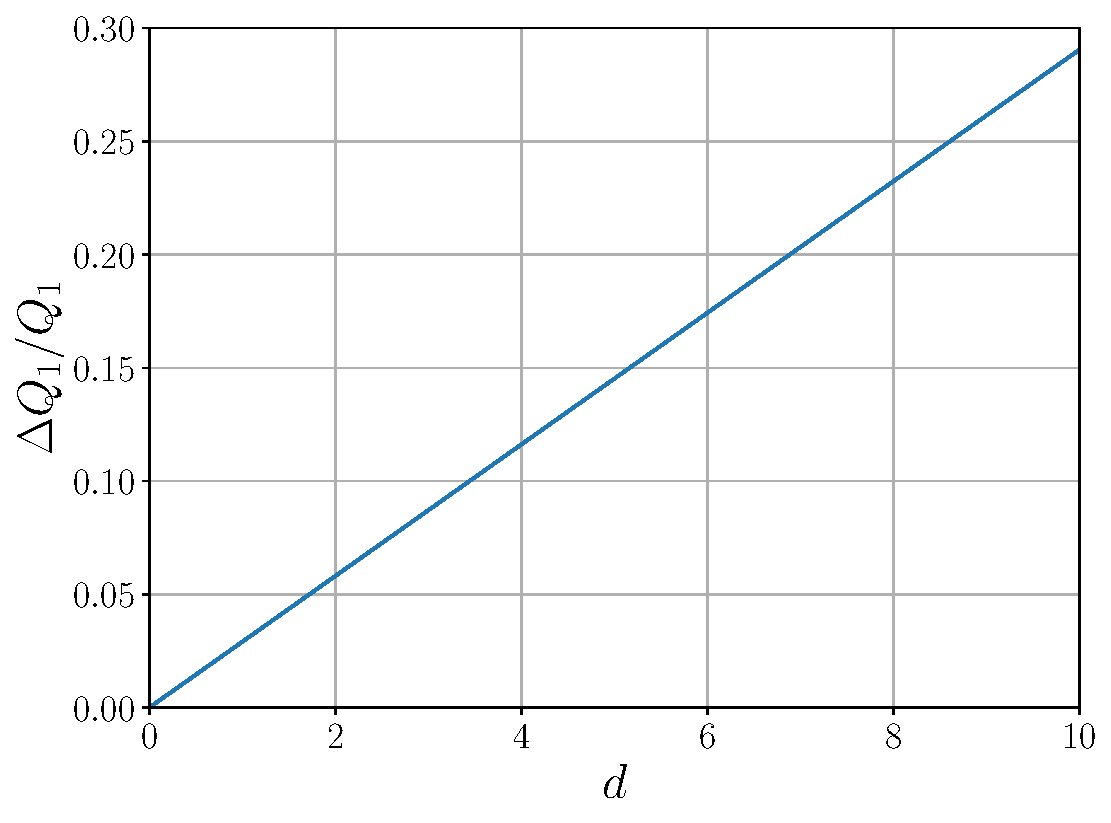
\includegraphics[width=5.0in]{figures/fret_disp}\caption{Relative displacement $\Delta Q_1 / Q_1$}
%         \label{fig:fret_disp}
%     \end{subfigure}
%     \par\vspace{0.25in}
%     \begin{subfigure}[b]{0.8\textwidth}
%         \centering
%         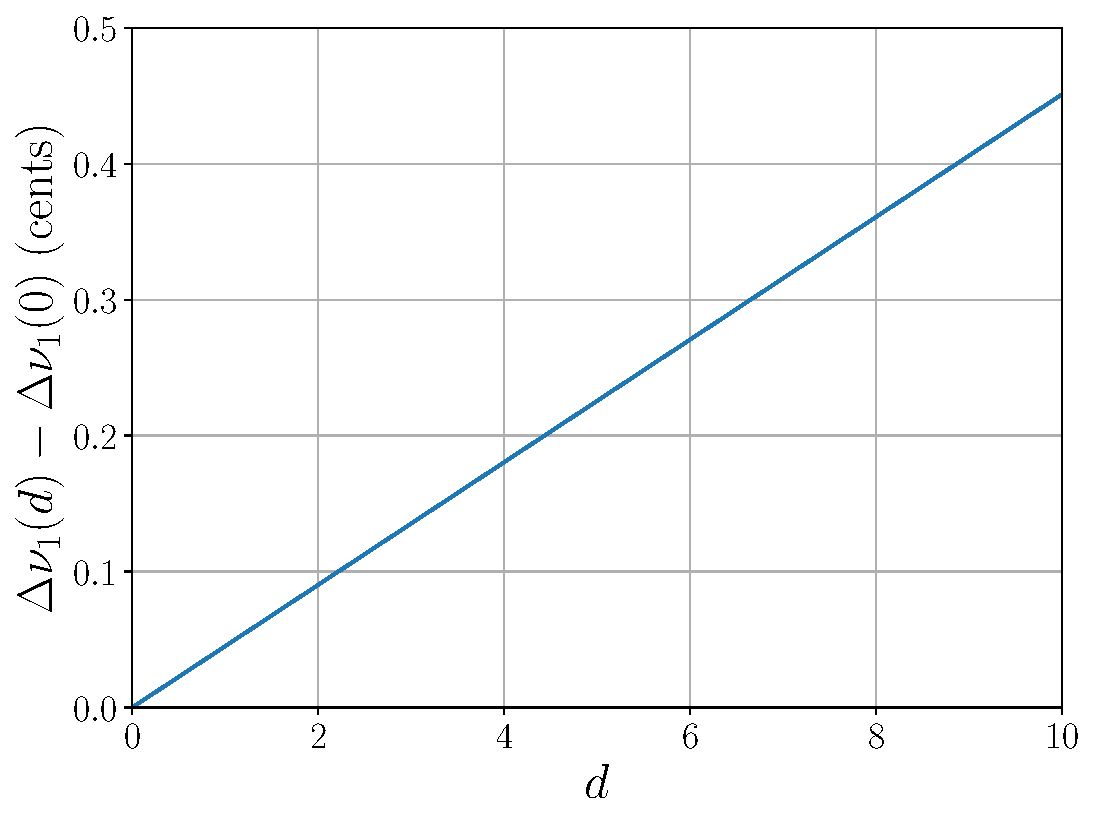
\includegraphics[width=5.0in]{figures/fret_shift}\caption{Additional frequency shift for $\kappa = 49$}\label{fig:fret_shift}
%     \end{subfigure}
%     \caption{\label{fig:fret_model} In (a), we plot the relative displacement $\Delta Q_1 / Q_1$ for the first fret as a function of the fretting distance parameter $d$ using \eqn{delta_q_n_approx}. Here the guitar has the same parameters as the ``no-relief'' Alhambra 8P, with normal tension strings. In (b), we show the additional frequency shift given by \eqn{delta_nu_n_d} at the first fret of a string with $\kappa = 49$ as $d$ increases from 0. For $n > 1$, the relative displacement and additional shift are reduced by a factor of approximately $n^2$.}
% \end{figure}
